\chapter{Теоретическая часть}\label{ch:ch1}

\section{Cреда выполнения}\label{sec:ch1/sec1}
Среда выполнения\footnote{(англ. execution environment, иногда «рантайм» от англ. runtime — «время выполнения»)} в информатике — вычислительное окружение, необходимое для выполнения компьютерной программы\cite{runtime}. 

К программной cреде робота предьявляются следующие требования:
\begin{enumerate}[beginpenalty=10000] % https://tex.stackexchange.com/a/476052/104425
  \item Деление на микропрограммы: должно быть чёткое разделение ответственности среди множества управляющих роботом компонентов;
  \item Единый стандарт общения между программами: это необходимо для корректного общения компонент;
  \item Синхронизация по времени: каждое сообщение, которым обмениваются микропрограммы должно сопровождаться временем его отправки чтобы у остальных компонент было понятие о времени отправки сообщения;
  \item Наличие общей среды для коммуникации: отправляющая сторона не должна иметь представление о том, куда ей отправить свои данные, а принимающая сторона о том, от кого эти данные взять;
  \item Управление данными: все приходящие данные нужно принять, все отправленные --- доставить. Слишком старые данные необходимо уничтожать чтобы не вызвать перегрузку на мобильном компьютере, которым оснащён робот.
\end{enumerate}

\section{Необходимые данные}\label{sec:ch1/sec2}

Для работы управляющей нейронной сети, которая не является частью данной работы, необходимы входные данные. К этим данным относятся:
\begin{enumerate}[beginpenalty=10000] % https://tex.stackexchange.com/a/476052/104425
  \item Текущее окружение робота в виде массива, элементами которого являются два значения: угол и расстояние до ближайшего препятствия;
  \item Изображение с видеокамеры робота для распознавания опасных объектов.
\end{enumerate}

На основе этих входных данных нейронная сеть должна предоставлять управляющий сигнал, который должен быть преобразован в команды для движения двигателей робота.

\section{Аппаратная часть робота}\label{sec:ch1/sec3}

К аппаратной части робота предьявляются следующие требования:
\begin{enumerate}[beginpenalty=10000] % https://tex.stackexchange.com/a/476052/104425
  \item Шасси должно быть как можно более мобильным, компактным и способно самостоятельно передвигаться;
  \item Вычисления должны проходить автономно на компьютере NVIDIA Jetson Xavier NX;
  \item Робот должен быть оснащён сканером окружающего пространства и уметь обнаруживать препятствия на любой стороне платформы;
  \item Видеокамера должна находиться по центру в передней части робота и иметь разрешение изображения не менее 720x720 пикселей.
  \item Компоненты не должны иметь высокую рыночную стоимость в следствии финансовых ограничений на данную работу.
\end{enumerate}

\section{NVIDIA Jetson Xavier NX}
Для разработки робота учебным учреждением был выделен одноплатный компьютер NVIDIA Jetson Xavier NX, изображённый на Рисунке~\cref{fig:xavier}~\cite{xavier}.

\begin{figure}[ht]
    \centerfloat{
        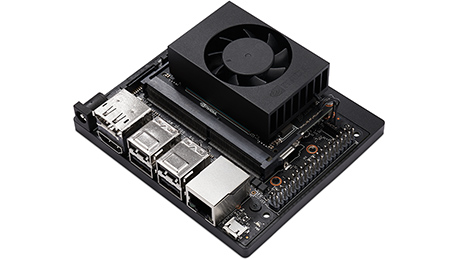
\includegraphics[scale=0.7]{xavier}
    }
    \caption{Внешний вид компьютера NVIDIA Jetson Xavier NX}\label{fig:xavier}
\end{figure}

Данный компьютер обладает следующими важными характеристиками~\cite{xavier}:

\begin{enumerate}[beginpenalty=10000] % https://tex.stackexchange.com/a/476052/104425
  \item GPU NVIDIA Volta™ с 384 ядрами CUDA и 48 тензорными ядрами;
  \item Шестиядерный 64-разрядный процессор NVIDIA Carmel с архитектурой ARM®v8.2;
  \item Оперативная память размером 8 ГБ типа LPDDR4x;
  \item Регулируемое энергопотребление: 10, 15 и 20 Вт;
  \item Интерфейс для подключения 2 CSI камер;
  \item 4 USB разъёма версии 3.0;
  \item Разъём GPIO с возможностью подключать устройства I2C;
  \item Размер платы составляет 103x90.5x31 мм.
\end{enumerate}

\FloatBarrier
